\documentclass{beamer}

\usepackage{fontenc}
\usepackage{listings,newtxtt}
\lstset{basicstyle=\tiny, keywordstyle=\bfseries}

\usepackage{xcolor}

\usepackage{subcaption}
\usepackage{adjustbox}

\graphicspath{{images/}}



\defbeamertemplate*{title page}{customized}[1][]
{
  \begin{center}
    \usebeamerfont{institute}\Huge\insertinstitute\par      
  \end{center}
  \centering
  \usebeamerfont{title}\LARGE\inserttitle\par
  \usebeamerfont{subtitle}\Large\insertsubtitle\par
  \bigskip
  \small\usebeamerfont{author}\insertauthor\par
  \usebeamerfont{date}\insertdate\par
}

\institute{Alma Mater Studiorum \\ University of Bologna}
\title{Artificial Intelligence - Computer vision}
\subtitle{Intrusion detection project}
\author{Alessandro Dicosola [Matr. 935563]}
\date{}

\definecolor{applegreen}{rgb}{0.55, 0.71, 0.0}

\definecolor{darkmagenta}{rgb}{0.55, 0.0, 0.55}

\begin{document}
 
\begin{frame}
    \titlepage
\end{frame}

\begin{frame}{Introduction}{Problem}
    Build an intrusion detection system using a static background as a reference
\end{frame}
\begin{frame}[fragile]{Introduction}{What is a pipeline?}
    \framesubtitle{What is a pipeline?}
    A sequence of transformations and operations
    \begin{columns}
        \begin{column}[t]{0.45\textwidth}
            \centering
            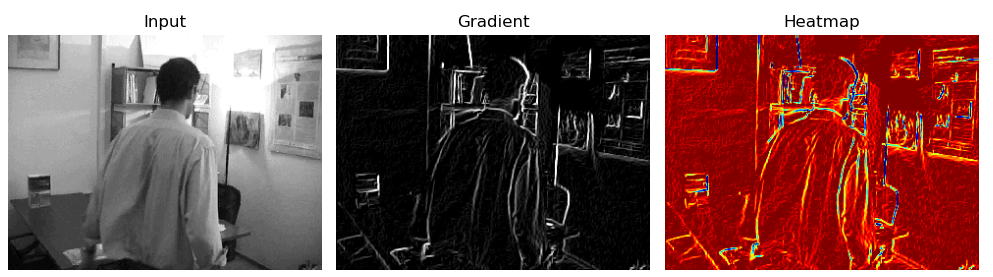
\includegraphics[width=150pt,keepaspectratio]{pipelineex1.png}
            \begin{lstlisting}[basicstyle=\tiny,breaklines=true,linewidth=150pt,language=Python]
pipeline.add_operation("Input", lambda frame: frame)
pipeline.add_operation("Gradient", lambda frame: get_grad(frame))
pipeline.add_operation("Heatmap", lambda frame: cv2.applyColorMap(frame, cv2.COLORMAP_JET))
            \end{lstlisting}
        \end{column}
        \begin{column}[t]{0.45\textwidth}
            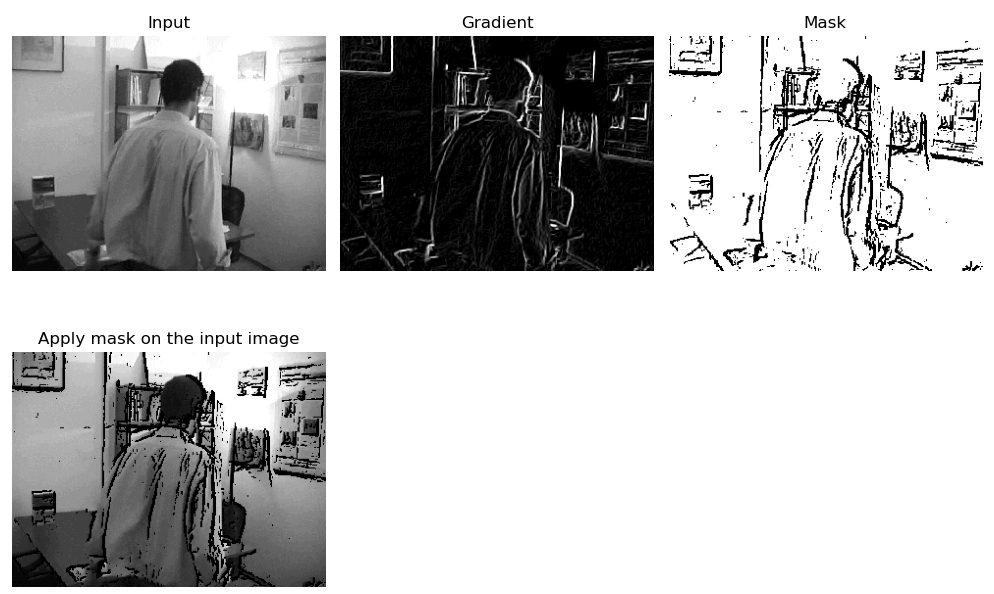
\includegraphics[width=150pt,keepaspectratio]{pipelineex2.png}
            \begin{lstlisting}[basicstyle=\tiny,breaklines=true,linewidth=150pt,language=Python]
pipeline.add_operation("Input", lambda frame: frame)
pipeline.add_operation("Gradient", lambda frame: get_grad(frame))
pipeline.add_operation("Mask", lambda frame: frame < 30)
def showonlymask(mask):
    import numpy as np
    input = pipeline.input.copy()
    out = np.empty_like(input)
    out[mask] = input[mask]
    return out

pipeline.add_operation("Apply mask on the input image", showonlymask)
            \end{lstlisting}
        \end{column}
        \begin{column}[t]{0.45\textwidth}
            
        \end{column}
    \end{columns}
\end{frame}

\begin{frame}{Preprocessing}{Gaussian blur}
    \begin{figure}
        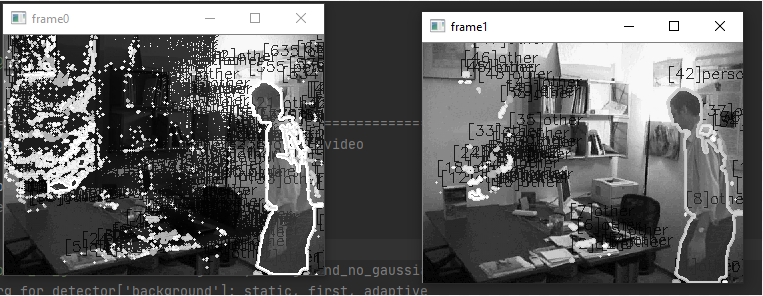
\includegraphics[width=\linewidth,keepaspectratio]{background_no_gaussian.PNG}
    \end{figure}
\end{frame}

\begin{frame}{Preprocessing}{Median filter}
    \begin{figure}
        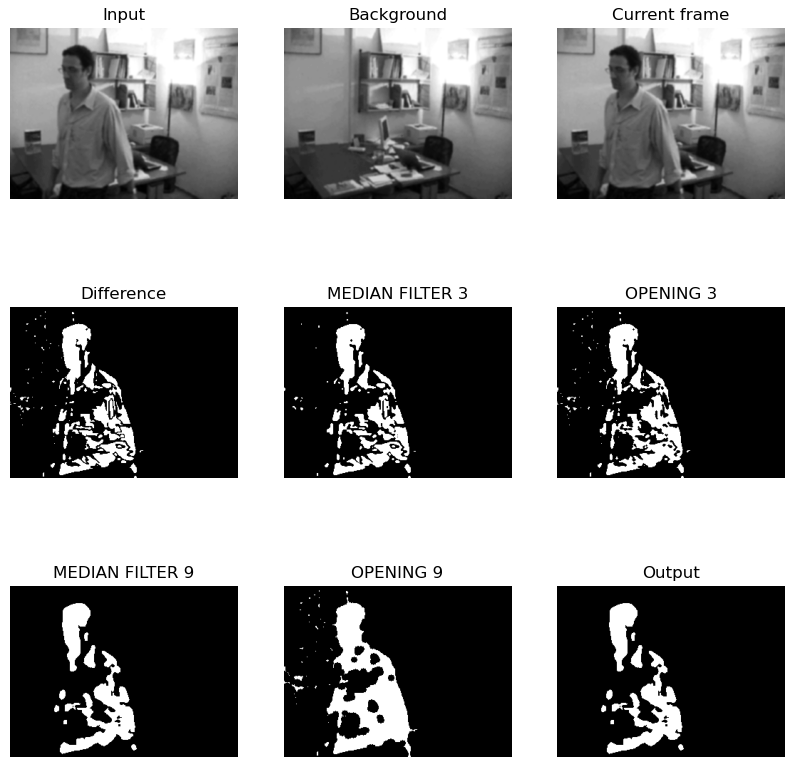
\includegraphics[width=0.7\textwidth,keepaspectratio]{median filter.png}
    \end{figure}
\end{frame}


\begin{frame}{Detector}{Background subtractor}
    \begin{itemize}
        \item Use a \textbf{static} background\
        \item Use the interpolation of the \textbf{first} 100 frames
        \item Use an \textbf{adaptive} background that computes the weighted sum of the current frame and the previous one
    \end{itemize}
\end{frame}



\begin{frame}{Detector}{Pipeline - static, first}
    \begin{figure}
        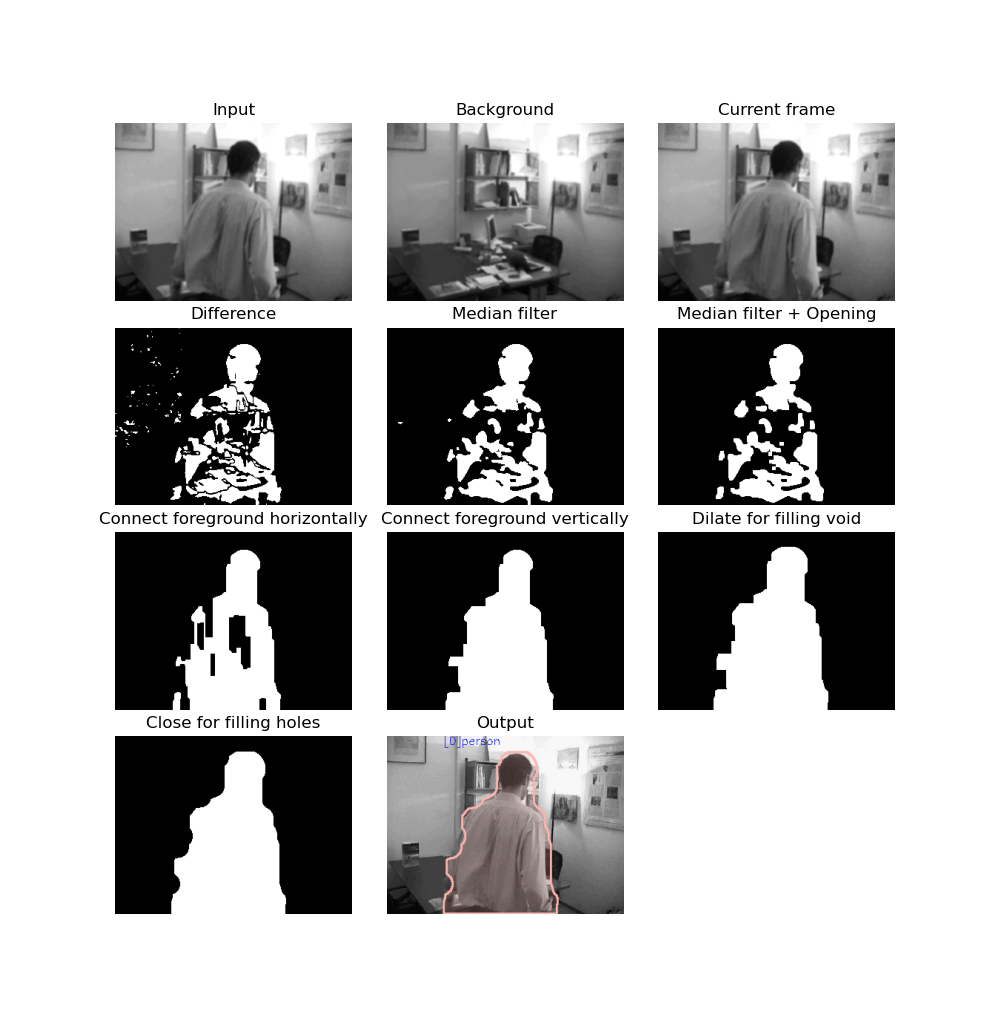
\includegraphics[height=0.9\textheight,keepaspectratio]{pipeline_Static_first.png}
    \end{figure}
\end{frame}

\begin{frame}{Detector}{Pipeline - adaptive}
    \begin{figure}
        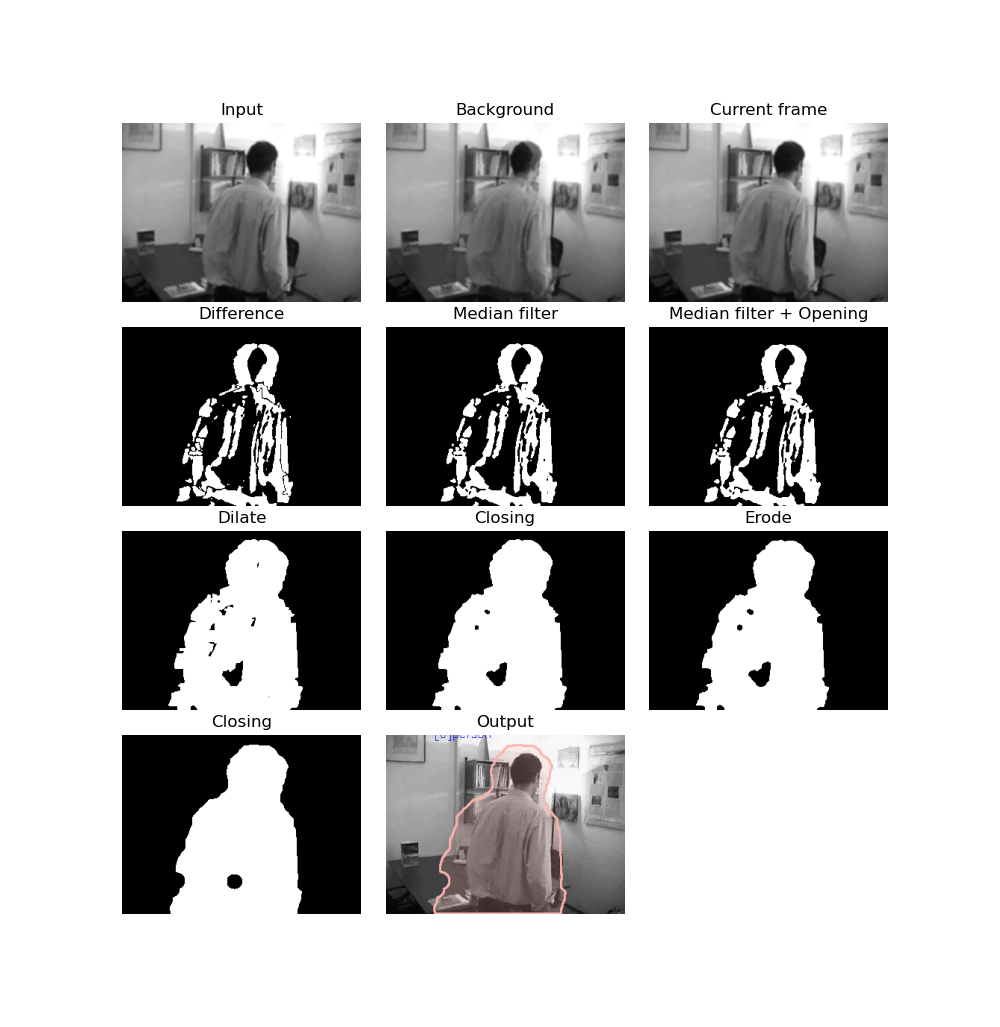
\includegraphics[height=0.9\textheight,keepaspectratio]{pipeline_adaptive.png}
    \end{figure}
\end{frame}

\begin{frame}[fragile]{Detector}{Parameters}
    \begin{tabular}{cccc}
        kind     & distance      & threshold & alpha\footnotemark \\
        \hline
        static   & max\_distance & 30        & -     \\
        first    & max\_distance & 34        & -     \\
        adaptive & l1            & 5         & 0.70
    \end{tabular}
    \footnotetext{alpha regulates the update speed (how fast the accumulator "forgets" about earlier images).}
\end{frame}

\begin{frame}{Detector - first}{Difference between threshold 30 and 34}
    \begin{columns}
        \begin{column}[t]{0.5\paperwidth}
            \centering
            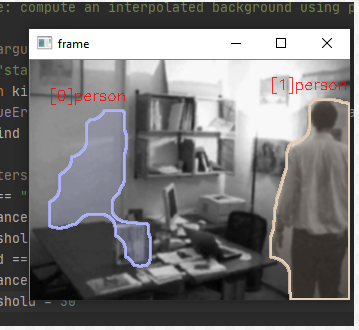
\includegraphics[width=0.5\textwidth,keepaspectratio]{background_first_30.PNG}
        \end{column}
        \begin{column}[t]{0.5\paperwidth}
            \centering
            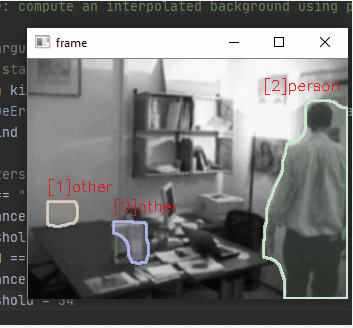
\includegraphics[width=0.5\textwidth,keepaspectratio]{background_first_34.PNG}
        \end{column}
    \end{columns}
\end{frame}

\begin{frame}{Detector - adaptive}{alpha parameter}
    \begin{columns}
        \begin{column}[t]{0.5\textwidth}
            \centering
            ALPHA = 0.7    
            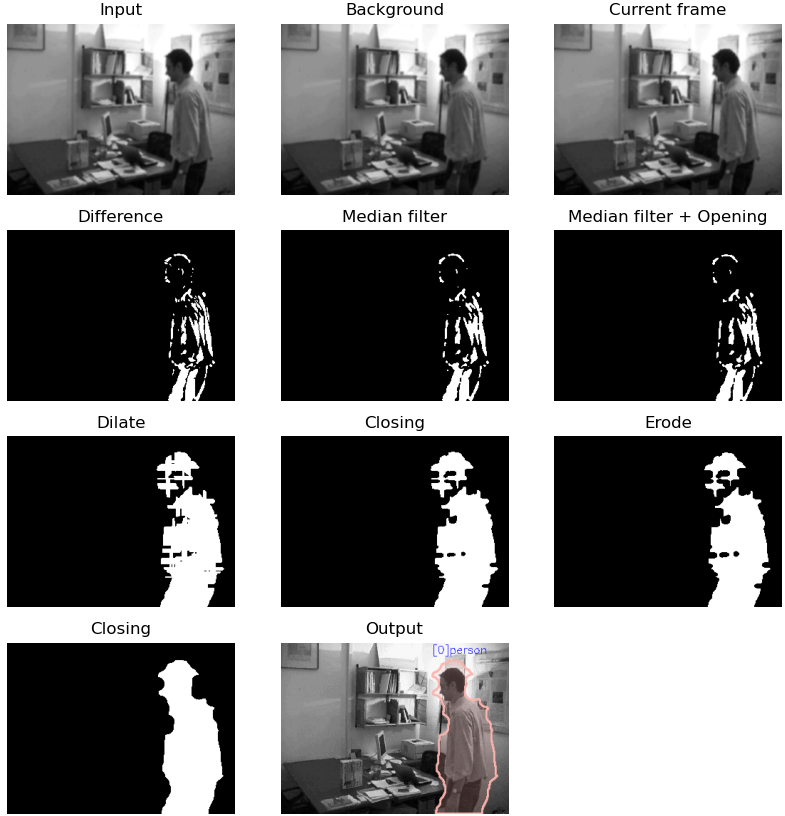
\includegraphics[width=120pt,keepaspectratio]{adaptive_alpha07_f482.png}
        \end{column}
        \begin{column}[t]{0.5\textwidth}
            \centering
            ALPHA = 0.8    
            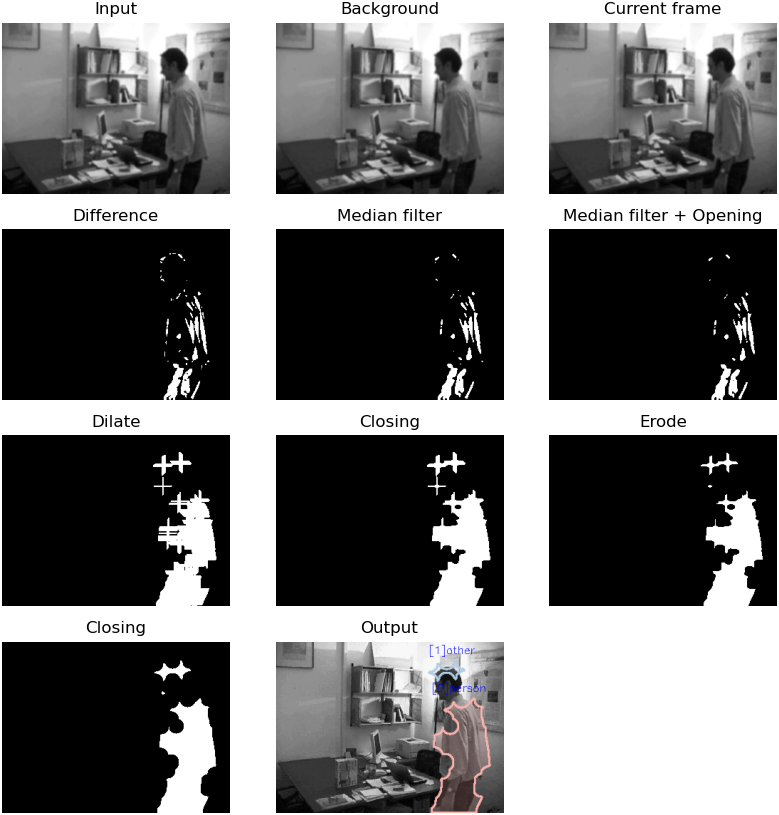
\includegraphics[width=120pt,keepaspectratio]{adaptive_alpha08_f482.png}
        \end{column}
    \end{columns}
\end{frame}

\begin{frame}[fragile]{Detector}{Filtering and handling false positive}
\tiny
\hspace*{-1cm}\begin{tabular}[h]{ccccccccc}
index & area	& perimeter & 	ratio & circularity & rectangularity & mean & std & label \\
0 & \color{orange}{1243.0} & \color{orange}{146.76} & 0.80 & 0.93 & \color{red}{1545.35} & 0.13 & 0.203 & other \\
1 & 855.0 & 113.45 & 1.06 & 1.06 & 803.18 & 0.013 & \color{darkmagenta}{0.020} & other false positive \\
2 & \color{applegreen}{15028.5} & 587.80 & \color{blue}{0.47} & 0.93 & 31897.22 & 0.09 & 0.177 & person
\end{tabular}        


\begin{columns}
    \begin{column}[t]{0.33\textwidth}
        \centering
        Filtering
        \begin{verbatim}
            rectangularity > 5000:
            else
            perimeter > 100 and area > 300
        \end{verbatim}        
    \end{column}
    \begin{column}[t]{0.33\textwidth}
        \centering
        Labelling
        \begin{verbatim}
            area > 3000 or ratio < 0.3            
        \end{verbatim}
    \end{column}
    \begin{column}[t]{0.33\textwidth}
        \centering
        False positive
        \begin{verbatim}
            std < 0.1
        \end{verbatim}
    \end{column}

\end{columns}
\end{frame}

\begin{frame}{Conclusion}{Output of the frame 481}
    \begin{columns}
        \begin{column}[t]{0.33\textwidth}
            \centering
            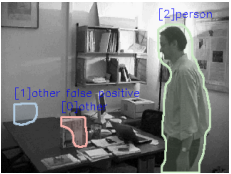
\includegraphics[width=\linewidth]{out481_static.PNG}
            static
        \end{column}
        \begin{column}[t]{0.33\textwidth}
            \centering
            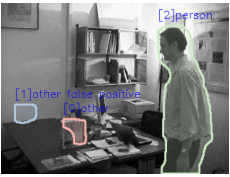
\includegraphics[width=\linewidth]{out481_first.PNG}
            first
        \end{column}
        \begin{column}[t]{0.33\textwidth}
            \centering
            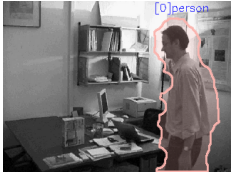
\includegraphics[width=\linewidth]{out481_adaptive.PNG}
            adaptive
        \end{column}
    \end{columns}
\end{frame}


        

\end{document}